\section{Zielsetzung}
    Das Ziel dieses Versuchs ist es die Rubidium-Isotope $\ce{^{85}Rb}$ und $\ce{^{87}Rb}$ mittels Hochfrequenzspektroskopie zu untersuchen.\\
    Dafür werden Elektronen durch optisches Pumpen in angeregte Zustände versetzt. Diese Zustände lassen sich dann mittels radio-frequenten magnetischen Feldern untersuchen.
\section{Theorie}

\subsection{Energielevelstruktur des Rubidium-Atoms}


\subsubsection{Die einfachen Niveaus und die Feinstruktur}
\noindent
Das Rubidium-Atom gehört zu ersten Hauptgruppe. Das Heißt, dass es nur ein Elektron in der äußersten Schale besitzt.\\
Dies macht es sehr geeignet für diesen Versuch, da damit nur ein Elektronenspin beachtet werden muss.\\
Der Unterschied zwischen den beiden Isotopen sind ihre Kernspins $I$. 
$\ce{^{85}Rb}$ hat einen Kernspin von $I = \frac{5}{2}$ und $\ce{^{87}Rb}$ von $I = \frac{3}{2}$.\\ 
Der Aufbau inklusive Spins ist auch in Abbildung \ref{img:Iso} noch einmal dargestellt.

\begin{figure}[H]
    \centering
    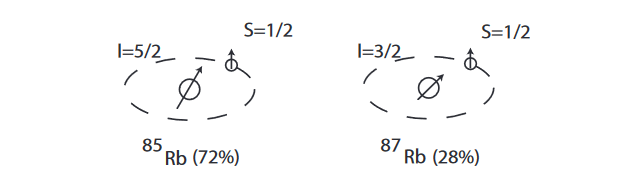
\includegraphics[width=0.6\textwidth]{latex/images/Isotopes.PNG}
    \caption{Die Rubidium-Isotope und ihre Spins schematisch dargestellt\protect \cite{pump_1}.}
    \label{img:Iso}
\end{figure}

\noindent
Die Energieniveaus des Valenzelektrons hängen in 1. Ordnung von der Hauptquantenzahl $n$ ab, welche beschreibt im wievielten angeregten Zustand sich das Elektron befindet.\\
Für jeden dieser Zustände kann dieser kann das Elektron unterschiedliche Bahndrehimpulse annehmen. Genauer gilt $l \in [0, n-1]$. Im Grundzustand gilt also $l = 0$.\\
Dieser Effekt hat die größten Energiedifferenzen $\increment E$ zwischen seinen Niveaus.\\\\
Dies sind aber nicht alle Effekte die zur Aufspaltung der Energieniveaus des Elektrons beitragen.
Des Weiteren muss noch beachtet werden, dass der Elektronenspin $s =\frac{1}{2}$ an seinen Bahndrehimpuls koppelt.\\
Dies ist die sogenannte $LS$-Kopplung oder Feinstruktur. \\
Stark vereinfacht gesagt wechselwirkt der Elektronenspin mit dem Magnetfeld, dass durch seine Bewegung entsteht, wodurch sich die Energieniveaus in $s$ und $l$ aufspalten.\\
Die Aufspaltung kann dabei durch $J$ den Spin der gesamten Schale beschrieben werden. Dabei kann $J$ Werte von $\bigl| L - S \bigr|$ bis $\bigl| L + S \bigr|$ annehmen.\\
Im Vergleich mit den $n$-Niveaus sind die Energiedifferenzen deutlich kleiner.\\
Im Versuch wird die Aufspaltung im Grundniveau $S_{\frac{1}{2}}$ und im ersten angeregten Zustand $P_\frac{1}{2}$ betrachtet.\\
Die Aufspaltung in der Feinstruktur und die weiteren Aufspaltungen in der Hyperfeinstruktur und dem Zeeman-Effekt sind in Abbildung \ref{img:aufspaltung} dargestellt.
\begin{figure}[H]
    \centering
    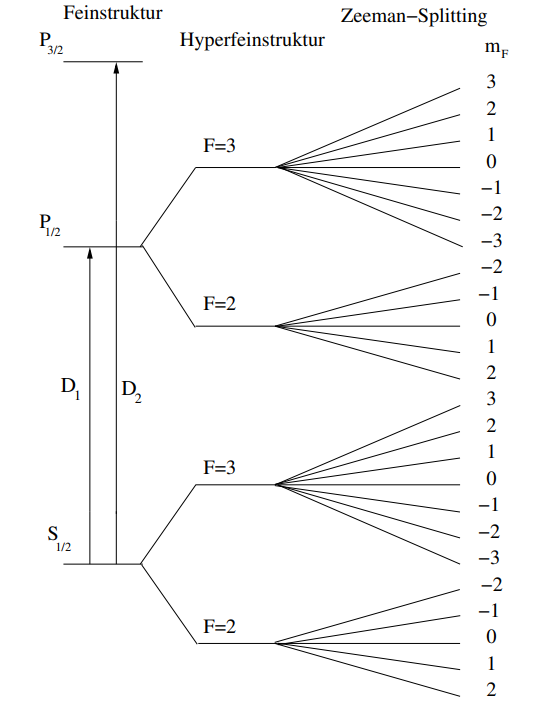
\includegraphics[width=0.5\textwidth]{latex/images/energy_levels_85.PNG}
    \caption{Die Aufspaltung der Energieniveaus von $\ce{^{85}Rb}$ in der Feinstruktur, Hyperfeinstruktur und unter dem Zeeman-Effekt.\\
    Die Indices der Energieniveaus stehen für die Werte von $J$ die angenommen werden \protect \cite{pump_2}.}
    \label{img:aufspaltung}
\end{figure}

\subsubsection{Die Hyperfeinstruktur und der Zeeman-Effekt}

\noindent
Ein zusätzlicher Effekt, der zu einer noch feineren Aufspaltung in den Energien führt, ist die Hyperfeinstruktur.\\
Sie entsteht daraus, dass der Gesamtspin des Atoms $F$ die Eigenwerte $\bigl| I - J \bigr|$ bis $\bigl| I + J \bigr|$ besitzt.\\
Je nach Wert des Bahndrehimpulses $J$ und des Kernspins $I$, ist die Wechselwirkung energetisch günstiger oder ungünstiger, wodurch unterschiedliche Energieniveaus entstehen.\\
Abbildung \ref{img:aufspaltung} zeigt dies für $\ce{^{85}Rb}$.\\\\

\noindent
Wenn nun noch ein externes Magnetfeld angelegt wird, tritt noch eine weitere Aufspaltung auf.\\
Dies ist der sogenannte Zeeman-Effekt und er hebt die Entartung der Energie in der magnetischen Quantenzahl $m$ auf.\\
Diese Quantenzahl beschreibt dabei die Projektion des Spins auf das externe Magnetfeld. 
Je nach Orientierung des Atomspins ist die Stärke der Kopplung zwischen magnetischem Moment und Magnetfeld also unterschiedlich.\\
$m$ hat dabei die $2F+1$ Eigenwerte von $-F$ bis $F$.\\
Für kleine externe Magnetfelder $B$  ergeben sich die Zeeman-Niveaus zu 
\begin{equation}
    E_Z = g_F \mu_B \bigl| B \bigr| m \quad .
    \label{eqn:zeeman}
\end{equation}
Sie beschrieben dabei die Abweichung von den Hyperfein-Niveaus in Abhängigkeit von der Stärke des Magnetfelds $\bigl| B \bigr|$, 
der magnetischen Quantenzahl $M$, dem Bohrschen Magneton $\mu_b$ und dem gyromagnetischen Verhältnis, oder Landé-Faktor $g_F$.\\
Der Landé-Faktor $g_F$ ist dabei nicht der des Elektrons. Für ihn gilt
\begin{align*}
    g_F &= g_J\frac{F(F+1) + J(J+1) - I(I+1)}{2F(F+1)}\\
    \intertext{mit}
    g_J &= 1 + \frac{J(J+1) + S(S+a) -L(L+1)}{2J(J+1)} \quad .
\end{align*}
Das Bohrsche Magneton setzt sich aus 
\begin{equation*}
    \mu_b = \frac{\symup e \symup \hbar}{2\symup{m_e}}
\end{equation*}
zusammen. $\symup e$  ist die Elektronenladung\cite{e0}, $\symup \hbar$ das reduzierte Plancksche Wirkungsquantum\cite{Planck} und $\symup{m_e}$ die Elektronenmasse\cite{m_e}.

\subsubsection{Der quadratische Zeeman-Effekt}

\noindent
In Anwesenheit schwacher Magnetfelder ist der Hamilton-Operator des Zeeman-Terms diagonal und seine Energieeigenwerte lassen sich durch Gleichung \ref{eqn:zeeman} ausdrücken.\\
Für sehr starke Magnetfelder wird der auftretende Effekt Paschen-Back-Effekt genannt. Dieser besitzt wieder einen diagonalisierten Hamilton-Operator. Allerdings in einer anderen Basis.\\
In der Übergangsregion der beiden Effekten sind daher noch zusätzliche quadratische Terme vonnöten um die Energieniveaus anzunähern.\\
Dies führt zu 
\begin{equation*}
 E_{Z} = lalalaal  \quad . 
\end{equation*} 


\subsubsection{Das optische Pumpen}

\noindent
Zuallererst befinden sich die Rubidium-Atome im thermischen Gleichgewicht. 
Das heißt, dass die Valenzelektronen aller Atome einer Boltzmann-Verteilung folgen. 
Bei angeschaltetem Magnetfeld sind sie also so über die Zeeman-Niveaus verteilt.\\\\
Optisches Pumpen ist dabei nun die gezielte Erzeugung einer der Besetzungszahlen im thermischen Gleichgewicht, mit optischen Mitteln.\\
Der ganze Vorgang ist schematisch in Abbildung \ref{img:pumpitup} zu sehen.

\begin{figure}[H]
    \centering
    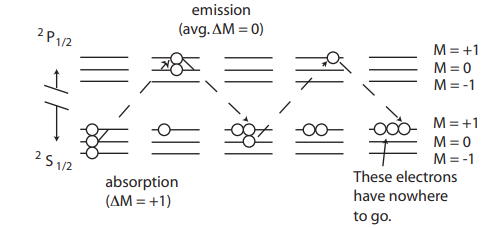
\includegraphics[width=0.6\textwidth]{latex/images/pumping.PNG}
    \caption{Der Ablauf des optischen Pumpens schematisch für das Wasserstoff-Atom dargestellt\protect \cite{pump_1}.}
    \label{img:pumpitup}
\end{figure}

\noindent
Für das Rubidium-Gas liegen die Hyperfein-Niveaus nah genug beieinander, als dass sie ziemlich ähnlich wahrscheinlich von Elektronen besetzt.\\
Es herrscht also gleiche Wahrscheinlichkeiten für alle $F$-Zustände mit jedem $m$.\\
Wenn ein Elektron nun von einem Photon angeregt wird, kann sich die Quantenzahl $m$ nur um $\pm 1$ oder gar nicht ändern.\\
Bei rechts zirkular polarisiertem Licht, welches sich parallel zum Magnetfeld ausbreitet, muss gelten $\increment m = +1$. 
Bei links zirkular polarisiertem Licht wäre es $\increment m = -1$ und bei linear polarisiertem $\increment m = 0$.\\
In diesem Fall wird das Rubidium-Gas mit recht zirkular polarisiertem Licht bestrahlt, welches die Energie des $D_1$-Übergangs besitzt.\\
Die Elektronen, die sich im Grundniveau $S_{\frac{1}{2}}$ der Feinstruktur befinden werden, dabei in den nächst höheren Zustand angeregt, 
das $P_{\frac{1}{2}}$-Niveau angeregt.\\
Dabei wird die magnetische Quantenzahl $m$ dann um $1$ erhöht. 
Dies geht natürlich nur für Werte von $m$, für die ein Zustand $m+1$ möglich ist.\\
Ist dieser Übergang nicht möglich können die Elektronen nicht angeregt werden.\\
Diesen Zustand verlässt das Elektron dann wieder, in dem es über spontane Emission ein Photon emittiert und in den Grundzustand zurückkehrt.
Dieses kann stochastisch jede Form haben und daher $m$ mit $\increment m = \pm 1,0$ ändern.\\
Mit der Zeit sammeln sich dann die Elektronen in den Zuständen, in denen sie nicht angeregt werden können.\\
Natürlich tritt bei diesem Vorgang auch induzierte Emission auf.
Das heißt, wenn ein Photon die Energie des Übergangs besitzt, kann es die Emission bei einem angeregten Elektron die Emission eines anderen Photons induzieren.
Das emittierte Photon besitzt dabei dieselben Eigenschaften wie das induzierende. Bei diesem Vorgang fällt das Elektron wieder in seinen Ausgangszustand zurück.\\
Da das Photon aber auch rechts zirkular polarisiert ist, gilt $\increment m = -1$, wodurch es wieder in seinem Ausgangszustand landet.\\
Dieser Vorgang verzögert also nur das optische Pumpen, verhindert es aber nicht.


\begin{figure}[H]
    \centering
    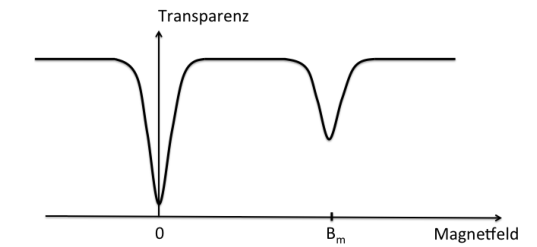
\includegraphics[width=0.6\textwidth]{latex/images/transp_plot.PNG}
    \caption{Eine Skizze des Plots, der die Transparenz des Gases gegen das Magnetfeld aufträgt. 
            Besonders zu beachten ist dabei der Transparenzabfall bei $B_m$\protect \cite{V21}.}
    \label{img:transp}
\end{figure}

\noindent
Das Gas ist also nun transparent. 
Diese Eigenschaft kann es nur verlieren, wenn die Elektronen wieder einen Zustand annehmen, aus dem heraus sie angeregt werden können.\\
Dies könnte wieder über spontane Emission geschehen, wobei in ein anderes Zeeman-Niveau gewechselt wird.
Die Wahrscheinlichkeit dieses Übergangs ist allerdings proportional zu $\nu ^3$ und daher hier zu vernachlässigen.\\
Alternativ könnte das Magnetfeld abgeschaltet werden, wodurch keine Zeeman-Aufspaltung mehr auftritt und $m$ daher keine relevante Quantenzahl mehr wäre.
Das Gas wäre dann wieder intransparent.\\
Wenn nun aber ein Magnetfeld angelegt werden wird, mit der Frequenz des Übergangs der Zeeman-Niveaus, würde die induzierte Emission auftreten.
Dabei würden die Elektronen wieder über die Zustände verteilt und das Gas undurchsichtig.\\
Es muss also gelten 
\begin{align}
    \omega_{RF} &= \frac{g_F \mu_B}{\hbar} \cdot \bigl| B_m \bigr| \\
    \label{eqn:freq} \notag
    \intertext{oder}
    \bigl| B_m \bigr|  &= \frac{\hbar \cdot \omega_{RF}}{g_F \mu_B} \quad . \notag
\end{align}
Mit $\omega_{RF}$ als Frequenz des radio-frequenten Magnetfeldes.\\
Diese Abhängigkeit ist in Abbildung \ref{img:transp} schematisch dargestellt.